\documentclass[../qm.tex]{subfiles}
\begin{document}
\section{First Discoveries}
At the end of the '800s we managed to discover radioactivity, and it was divided as follows
\begin{itemize}
\item X rays, discovered by Röntgen in 1895
\item Natural radioactivity observed in phosphorescent materials as ${}^{238}$U salts, of which
	\begin{itemize}
	\item $\alpha$ rays
	\item $\beta$ rays
	\item $\gamma$ rays
	\end{itemize}
\end{itemize}
The firsts, X-rays, were known for passing easily through matter and leave traces in photographic tables, they're now known as high energy photons\\
The last, natural radiation in the shape of $\alpha,\beta$ and $\gamma$ radiation are now today known as emission of particular particles by atomic nuclei
\begin{enumerate}
\item $\gamma$ rays, today known as photons for which $E>E_X$
\item $\beta$ rays, today known as electrons and their antimatter counterpart, the positron
\item $\alpha$ rays, now known as Helium nuclei, which are emitted only from heavy nuclei
\end{enumerate}
\subsection{Thompson and the Discovery of the Electron}
One of the first experiments was conducted by Thompson, Milliken et. al which studied the nature of $\beta$ particles using a CRT as in picture
\begin{figure}[H]
	\centering
	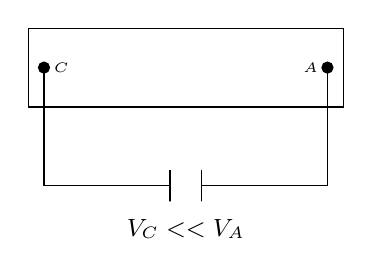
\begin{tikzpicture}
		\draw (-2,-0.5) rectangle (2,0.5);
		\draw[fill=black] (-1.8,0) circle (2pt);
		\draw[fill=black] (1.8,0) circle (2pt);
		\node[right] at (-1.8,0) (c) {\tiny$C$};
		\node[left] at (1.8,0) (a) {\tiny$A$};
		\draw (1.8,0) -- (1.8,-1.5) -- (0.2,-1.5) -- (0.2,-1.7) -- (0.2,-1.3);
		\draw (-1.8,0) -- (-1.8,-1.5) -- (-0.2,-1.5) -- (-0.2,-1.7) -- (-0.2,-1.3);
		\node[below] at (0,-1.8) (vcva) {\small$V_C<<V_A$};
	\end{tikzpicture}
	\caption{An example of a CRT's functioning, the cathode $C$ and the anode $A$ are enclosed in a glass tube}
	\label{fig:crt}
\end{figure}
The Thompson-Milliken experiment goes as follows: Filling the CRT tube with different gases it's possible to measure events in function of the kind of gas, its pressure, the potential difference $V_A-V_C$ and obviously in function of the material used to produce the cathode.\\
The observations that the scientists reported were
\begin{itemize}
\item A green luminescence close to the anodes
\item Electric shocks present also with small $\Delta V$
\item The electrical screening between the anode and cathode grows with $\Delta V$
\item All these effects are independent from the presence of a magnetic field $B$
\end{itemize}
They ended up with an hypothesis: CRT rays must be charged particles.\\
Thompson went forward proving this setting a new experiment, set up as in the following picture
\begin{figure}[H]
	\centering
	\begin{tikzpicture}
		\draw (-4.5,0) -- (-3,0);
		\draw[dashed] (-3,0) -- (5,0);
		\draw (-3,0) -- (-3,1) -- (-2.6,1) -- (-2.6,1.1) -- (-2.6,0.9);
		\draw (-2.4,0.7) -- (-2.4,1.3) -- (-2.4,1) -- (-1,1);
		\draw[pattern=north east lines] (-1,0.2) rectangle (-0.5,1.8);
		\draw[pattern=north east lines] (-1,-0.2) rectangle (-0.5,-1.8);
		\node[rectangle,fill=white,draw=white] at (-0.75,1) {\tiny$A$};
		\node[rectangle,fill=white,draw=white] at (-0.75,-1) {\tiny$A$};
		\draw[thick,dotted] (-0.5,1.8) -- (0,1.8);
		\draw[thick,dotted] (-0.5,-1.8) -- (0,-1.8);
		\draw (0,1.8) -- (3,1.8);
		\draw (0,-1.8) -- (3,-1.8);
		\draw[dotted] (0,0) ellipse (0.1 and 1.8);
		\draw (0,1.8) arc(90:270:0.1 and 1.8);
		\draw[dotted] (3,0) ellipse (0.1 and 1.8);
		\draw (3,-1.8) arc(270:90:0.1 and 1.8);
		\draw[->] (1.5,0) -- (1.5,1);
		\node[right] at (1.5,0.5) (e) {\tiny$\vec{E}$};
		\node[below] at (1.5,-0.5) (vx) {\tiny$v_x$};
		\draw[pattern=north east lines,draw=white] (5,-1.8) rectangle (5.5,1.8);
		\node at (5.25,0) [rectangle,draw=white,fill=white] (S) {\tiny$S$};
		\draw (5,1.8) -- (5,-1.8);
		\draw (5,1.8) -- (5.5,1.8);
		\draw (5,-1.8) -- (5.5,-1.8);
		\draw[->] (0,0) -- (5,-1.5);
		\draw[dashed] (3,1.8) -- (5,1.8);
		\draw[dashed] (3,-1.8) -- (5,-1.8);
		\draw[<->] (0,-2.2) -- (3,-2.2);
		\node at (1.5,-2.2) [rectangle,draw=white,fill=white] (l) {\tiny$L$};
		\draw[<->] (3,-2.2) -- (5,-2.2);
		\node at (4,-2.2) [rectangle,draw=white,fill=white] (dx) {\tiny$\Delta x$};
		\draw[<->] (5.8,0) -- (5.8,-1.5);
		\node at (5.8,-0.75) [rectangle,draw=white,fill=white] (ys) {\tiny$y_s$};
		\node at (-3,0) [circle,fill=white,draw=black] (c) {\tiny$C$};
	\end{tikzpicture}
	\caption{Scheme of the Thompson experiment. The electrons emitted from the cathode $C$ travel through a cylindrical capacitor long $L$ at a constant velocity $v_x$. Interacting with the electric field the path of the radiation variates and this variation is measured in a screen $S$ at the end}
	\label{fig:thompsonexp}
\end{figure}
In this experiment, we have $V_A>>V_C$ and therefore the electrons are accelerated from $C$ to $A$, from which continue traveling with constant velocity $v_x$. The $y$ component of the velocity gets perturbed by an electrostatic force, which gives us, inside the cylinder
\begin{equation}
	\left\{ \begin{aligned}
		a_x&=0\\
		a_y&=\frac{q}{m}E
	\end{aligned}\right.
	\label{eq:insidecapthom}
\end{equation}
Which implies
\begin{equation*}
	\left\{\begin{aligned}
		x(t)&=v_xt\\
		y(t)&=\frac{q}{2m}Et^2
	\end{aligned}\right.
\end{equation*}
Since the capacitor is long $L$ we have that when exiting the capacitor at a time $t_L=L/v_x$ the particle will be at the following $y$ position with $v_y$ velocity
\begin{equation*}
	\left\{ \begin{aligned}
			y(t_L)&=\frac{q}{2m}\frac{EL^2}{v^2_x}\\
			v_y(t_L)&=\frac{q}{m}\frac{EL}{v_x}
	\end{aligned}\right.
\end{equation*}
The final measured $y$ position on the screen, $y_s$ will be given by an easy computation
\begin{equation*}
	y_s=y(t_L)+v_y(t_L)\frac{\Delta x}{v_x}
\end{equation*}
Where $\Delta x$ is the horizontal distance between the end of the capacitor and the screen.\\
We get therefore
\begin{equation}
	y_s=\frac{qE}{2m}\frac{L^2}{v_x^2}+\frac{qE}{m}\frac{L\Delta x}{v_x^2}=\frac{qE}{m}\frac{L}{v_x^2}\left( \frac{L}{2}+\Delta x \right)
	\label{eq:yscreenthomp}
\end{equation}
The problem with this equation is that $v_x$ is unknown and therefore it's not possible to find $q/m$.\\
Accounting for an orthogonal magnetic field $B$ and applying the Lorentz force it's possible to find that
\begin{equation*}
	v_x=\frac{E}{B}
\end{equation*}
And therefore
\begin{equation}
	\frac{q}{m}=\frac{y_s}{L\left( \frac{L}{2}+\Delta x \right)}\frac{E}{B}
	\label{eq:qmelectron}
\end{equation}
This is a property of the projectile since it's invariant with the gas and the components of the anodes, and Nobel in 1906 calculated
\begin{equation*}
	\frac{q}{m}=1.76\cdot10^{11}\ \mathrm{C/kg}
\end{equation*}
A subsequent experiment by Milliken et al. in 1923 used a falling drop of oil in order to calculate the charge of this new particle.
The setup of the experiment was as follows
\begin{figure}[H]
	\centering
	\begin{tikzpicture}
		\draw (0,0) circle (0.5);
		\draw[->] (0,0) -- (0.35,0.35);
		\node[left] at (0.17,0.17) (r) {\tiny$r$};
		\draw[pattern=north east lines,draw=white] (-2,-2) rectangle (1.8,-1.5);
		\draw (-2,-1.5) -- (2,-1.5);
		\draw (1.8,-1.8) -- (1.8,1);
		\draw[->] (2,1) -- (2,0.5);
		\node[right] at (2,0.75) (g) {\tiny$\vec{g}$};
		\draw[dashed,->] (0,0) -- (0,-1);
		\node[right] at (0,-0.7) (v) {\tiny$\vec{v}$};
	\end{tikzpicture}
	\caption{Experimental setup of the falling droplet of oil}
	\label{fig:dropmilliken}
\end{figure}
This experiment used a falling drop of oil. The mass of the drop is quickly calculated assuming a spherical drop
\begin{equation*}
	m_p=\frac{4\pi}{3}r^3\rho_{oil}
\end{equation*}
Using hydrodynamics the drag force's modulus is quickly calculated accounting for the viscosity $\eta$ as follows
\begin{equation*}
	F_d=-6\pi\eta rv_0
\end{equation*}
Where $v_0$ is experimentally measured as the terminal velocity of the droplet. The classical equilibrium is reached when the weight of the droplet is balanced by the hydrodynamic drag
\begin{equation*}
	\frac{4\pi}{3}\pi r^3\rho_{oil}g=6\pi rv_0
\end{equation*}
Solving for $r$ we get a measurable formula for the radius of the droplet, i.e.
\begin{equation}
	r=\sqrt[3]{\frac{\eta v_0}{2\rho_{oil}g}}
	\label{eq:dynradoil}
\end{equation}
Applying now an electric field opposite to the motion of the droplet we get a new terminal velocity $v_1$ which can be experimentally measured, gives a relation between the known measured variables and the charge, as follows
\begin{equation*}
	qE=2\pi r\left( \frac{2r^2}{3}\rho_{oil} g-3\eta v_1 \right)
\end{equation*}
Substituting for $r$ and with some algebra we get
\begin{equation*}
	qE=18\eta\pi\sqrt{\frac{\eta v_0}{2\rho_{oil}g}}\left( v_0-v_1 \right)
\end{equation*}
Since $E$ is known and the variation in terminal velocities of the droplet is directly measured we get that the charge of this new particle is
\begin{equation}
	q=\frac{18\eta\pi}{E}\sqrt{\frac{\eta v_0}{2\rho_{oil}g}}\Delta v=1.59\cdot10^{-19}\ \mathrm{C}
	\label{eq:echargemill}
\end{equation}
The final value reached from Milliken is so precise that its relative error is in the $1\%$ from the modern known value.\\
Mixing the result of these two experiment it's possible to evaluate the mass of these beta particles, which gives
\begin{equation}
	m_\beta=0.911\cdot10^{-30}\ \mathrm{Kg}\approx511\ \mathrm{KeV}
	\label{eq:massbeta}
\end{equation}
This beta particle is now a well known fundamental particle that we treated already in depth in the previous chapters, which is the electron.
\subsection{Discovery of the Nucleus}
After the discovery of the electron and its properties with $\beta$ radiation, Rutherford et al. proceeded with a new experiment trying to discern the physics behind $\alpha$ particles. It was known that for some atom, with $A$ big enough, we can have a radioactive decay through the emission of an $\alpha$ particle, in the following reaction
\begin{equation}
	\nuc{N}{A}{Z}\to\nuc{M}{A'}{Z'}+\alpha
	\label{eq:alphadecruth}
\end{equation}
Note that today it's known that $\alpha=\nuc{He}{4}{2}$, $m_\alpha=3.7$ GeV and $A'=A-4$, $Z'=Z-2$.\\
These $\alpha$ particles emitted naturally by these heavy nuclei have a center of mass energy of around 5 MeV. Using special relativity we know that they aren't relativistic, in fact we have
\begin{equation*}
	E_{cm}=E_\alpha-m_\alpha=(\gamma-1)m_\alpha\implies\gamma\approx2.35\cdot10^{-3}
\end{equation*}
Rutherford's experiment was initially in order to determine which of the nuclear models was true. At the time there were two main contending ideas, one being Thompson's idea, where the electrons $q<0$ were situated inside this nucleus with $q_n>0$ and the total atom was neutral (the so called Pancake nucleus) whereas Rutherford supposed of an atom with the positive charges all in the center and electrons orbited these positive charges, rendering in general the atom neutral.\\
This experiment is extremely similar to the setup \eqref{fig:diffcsscat}, where the target is our nucleus with $q>0$.\\
The experimental setup that Rutherford et al. used consisted of a radioactive $\alpha$ emitter bar targeting these particles to a foil of gold $\nuc{Au}{}{79}$ which is surrounded by a $150^\circ$ spherical detector, which would measure the differences in the deflection angles.\\
The source chosen was Radium Bromide, $\mathrm{RaBr_2}$, an alpha emitter radioactive compound.
\begin{figure}[H]
	\centering
	\begin{tikzpicture}
		\draw[pattern=north east lines] (-1.5,-0.4) rectangle (1,0.4);
		\node at (-0.25,0) [rectangle,draw=white,fill=white] (rabr) {\small$\mathrm{RaBr_2}$};
		\draw[->] (1,0) -- (2,0);
		\node[below] at (1.5,0) (a) {\tiny$\alpha$};
		\draw[dashed] (1.5,0) -- (3.7,0);
		\draw[pattern=north east lines] (3.7,-0.7) rectangle (4.6,0.7);
		\node at (4.15,0) [rectangle,draw=white,fill=white] (au) {\small Au};
		\draw (6.2,0) arc(0:75:3cm);
		\draw (6.2,0) arc(0:-75:3cm);
	\end{tikzpicture}
	\caption{The setup was as follows, the radioactive source was placed at some distance from a gold plate at the center of a semi-spherical detector, which would then be used to determine the deviation angles of the deflected $\alpha$ particles}
	\label{fig:rutherfordsetup}
\end{figure}
The main scope of the experiment was to measure the numbers of reaction with respect to the deviation angle.\\
This can be done by firstly finding the differential cross section. The experimental setup makes it much easier since the spherical symmetry of the system easies the calculation.\\
Since the angular momentum of the particles and energy is conserved we can begin by writing the Lagrangian of the system
\begin{equation}
	\lag_\alpha=\frac{m_\alpha}{2}\left( \dot{r}^2+r^2\dot{\varphi}^2 \right)-\pot(r)
	\label{eq:rutherfordlag}
\end{equation}
Thanks to the spherical symmetry we have that $\dot{\varphi}$ is cyclical and its momentum will be conserved, i.e.
\begin{equation*}
	p_\varphi=mr^2\dot{\varphi}=L
\end{equation*}
And the energy of the system is
\begin{equation*}
	E=p\dot{q}-\lag_\alpha=\frac{1}{2}m_\alpha\dot{r}^2+\frac{1}{2}m_\alpha r^2\dot{\varphi}^2+\pot(r)
\end{equation*}
Substituting the cyclical coordinate with the conserved quantity $L$ we have
\begin{equation}
	E=\frac{1}{2}m\dot{r}^2+\frac{L^2}{2mr^2}+\pot(r)=T(\dot{r})+\pot_{eff}(r)
	\label{eq:effpotenruth}
\end{equation}
Where $\pot_{eff}(r)$ is an effective potential that includes the centrifugal potential.\\
Solving for $\dot{r}$ we get thanks to the conservation of energy the following differential equation
\begin{equation*}
	\dv{r}{t}=\sqrt{\frac{2}{m_\alpha}}\sqrt{E-\frac{L^2}{2mr^2}-\pot(r)}
\end{equation*}
In order to evaluate in terms of the deflection angle, using $p_\varphi$ we can substitute $\dd t$ with $\dd\varphi$, using the straightforward substitution
\begin{equation*}
	\dd\varphi=\frac{L}{m_\alpha r^2}\dd t
\end{equation*}
Which gives
\begin{equation*}
	\dd\varphi=\frac{\frac{L}{m_\alpha r^2}}{\sqrt{2m_\alpha}\sqrt{(E-\pot(r))-\frac{L^2}{r^2}}}\dd r
\end{equation*}
It's now useful to pass everything to the impact parameters for the $\alpha$ particle.\\
The conservation of energy permits us to write without problems that
\begin{equation}
	\left\{ \begin{aligned}
		p_i&=m_\alpha v_\infty\\
		E_\infty&=E_0=\frac{1}{2}m_\alpha v_\infty^2\\
		L&=\norm{r_\infty\wedge p_\infty}=bm_\alpha v_\infty
\end{aligned}\right.
	\label{eq:impactparruth}
\end{equation}
Where $r_\infty$ is the distance of the particle from the nucleus of gold, $v_\infty$ is the velocity ``at infinity'', i.e. the velocity of the non-interacting particle, and $b$ is the already known impact parameter.\\
Substituting into the differential of $\varphi$ we have that
\begin{equation*}
	2m_\alpha\left( \frac{1}{2}m_\alpha v_\infty^2-\pot(r)-\frac{b^2m^2v_\infty^2}{r^2}\right)=m^2_\alpha v^2_\infty\left( 1-\frac{\pot(r)}{E_\infty}-\frac{b^2}{r^2} \right)
\end{equation*}
Substituting it back and integrating we have
\begin{equation*}
	\varphi(r)=\int_{r_{min}}^{\infty}\frac{b}{r\sqrt{1-\frac{\pot(r)}{E_\infty}-\frac{b^2}{r^2}}}\dd r
\end{equation*}
The potential is the usual Coulomb potential, which in natural units is
\begin{equation*}
	\pot(r)=\frac{\alpha Z_pZ_n}{r}=\frac{A}{r}
\end{equation*}
Substituting it back into the integral we get a solvable integral
\begin{equation}
	\varphi(r)=\frac{r_{min}}{\infty}\frac{b}{r\sqrt{1-\frac{A}{E_\infty r}-\frac{b^2}{r^2}}}\dd r=\arccos\left[ \frac{\frac{A}{2E_\infty b}}{\sqrt{1+\left( \frac{A^2}{2E_\infty b} \right)}} \right]
	\label{eq:phirruth}
\end{equation}
Writing $B=A/2E_\infty b$ lets us invert the function in terms of the impact parameter, giving us
\begin{equation}
	b(\varphi)=\frac{A}{2E_\infty}\tan\left( \varphi \right)
	\label{eq:impactruth}
\end{equation}
It's quick to see that $\varphi=\pi/2-\theta/2$, therefore
\begin{equation}
	b(\theta)=\frac{A}{2E_\infty}\cot\left( \frac{\theta}{2} \right)
	\label{eq:bthetaruth}
\end{equation}
Deriving with respect to $\theta$ and inserting it into the equation for the differential cross section we get
\begin{equation}
	\dv{\sigma}{\Omega}=\frac{\alpha^2 Z_p^2Z_n^2}{16E_\infty^2}\csc^4\left( \frac{\theta}{2} \right)
	\label{eq:ruthcrosssec}
\end{equation}
Rutherford confirmed this cross section, and went forward estimating the value of $r_{min}$. Using $E_\infty=E_\alpha=5$ MeV and the conservation of energy we have
\begin{equation*}
	\pot(r_{min})=\frac{\alpha Z_pZ_n}{r_{min}}=\frac{1}{2}m_\alpha v_\infty^2=5\ \mathrm{MeV}
\end{equation*}
I.e.
\begin{equation*}
	r_{min}=\frac{\alpha Z_pZ_n}{5}\ \mathrm{MeV^{-1}}=0.23\ \mathrm{MeV^{-1}}
\end{equation*}
Converting into more usual units we have that $r_{min}=46$ fm, which from the experiment it was confirmed that $r_{min}<30$ fm.\\
\subsection{Discovery of the Proton and of the Neutron}
Again from Rutherford et al. in 1918, still using $\alpha$ radiation, the proton was discovered.\\
Consider the following nuclear reaction
\begin{equation*}
	\alpha+\nuc{N}{14}{7}\to\nuc{O}{17}{8}+X
\end{equation*}
This reaction included an artificial nuclear transmutation and the emission of an unknown particle $X$ on which a spectrography was executed and the measured $q/m$ was compatible with $\nuc{H^+}{}{}$. This particle was called the proton, with symbol $p$. The reaction was now completed
\begin{equation*}
	\alpha+\nuc{N}{14}{7}\to\nuc{O}{17}{8}+p
\end{equation*}
Continuing on this path, Chadwick et al. studied another reaction, for which an unknown neutral particle was discovered. The reaction is
\begin{equation*}
	\alpha+\nuc{Be}{9}{4}\to\nuc{C}{12}{6}+X
\end{equation*}
The creation of this particle was observed also with $\nuc{Li}{9}{4}$ and $\nuc{B}{9}{4}$
This particle is heavily piercing, and therefore two main hypotheses were considered
\begin{enumerate}
\item The particle is a photon
\item It's a new heavy neutral particle
\end{enumerate}
The idea for evaluating which is true was to consider the scattering with a proton from which to measure the impulse of $p$ and therefore evaluate the mass of this unknown particle.\\
The measured impulse of the proton after the scattering event had velocities $\beta\approx0.1$ and therefore can be considered weakly relativistic.\\
Curie et al. went forward proposing the idea that the $X$ particle was a photon with an energy of around 50 MeV, which tho contradicted previous experiments for which the energy of such photon would have been of the order of one MeV.\\
Chadwick et al. finally concluded that this was a new neutral massive particle, for which $m_n\approx m_p\pm10\%$. This particle was called the neutron, and is between the early fundamental blocks of nuclear physics together with $p$, $e^-$ and $\alpha$ particles.
\subsection{Modern Considerations and Experiments}
In our modern understanding of nuclear physics we know 7 main properties of atomic nuclei
\begin{itemize}
\item Mass $A$
\item Charge $Z$, number of protons
\item Number of neutrons $N=A-Z$
\item Nuclear spin
\item Magnetic moment $\mu$
\item Electric moments and quadrupole moments $'m$
\item Isospin
\end{itemize}
All the chemical properties are tied to the charge of the nucleus $Z$ and therefore compose the periodic table.\\
With these properties one can use the two main ones, $A,Z$ in order to build a couple and from there identify a nucleus. In general, a nuclear object with mass and charge $(A,Z)$ will be called a \emph{nuclide}.\\
An \emph{isotope} is a nuclide of some determined element $(A',Z)$ for which although the mass is different, the charge is the same. Vice-versa one can define \emph{isobars}, or a nuclide of some determined element $(A,Z')$ for which charge is different but the mass is the same.\\
The properties of a nucleus can be found out with different experiments.\\
Starting for mass one can repeat the Thompson experiment using a mass spectrometer, while for charge one can use an X ray spectroscopy of the internal electron shells of the atom. Other experiments include tests for finding the radius of a nuclide, repeating the Chadwick-Rutherford experiment with either highly energetic electrons in order to have a smaller resolution, or using $\mu$-mesic studies of the atom with muons instead of electrons, which all give finer details on the nucleus.\\
The final conclusion from all the various experiments are that
\begin{itemize}
\item The matter distribution is proportional to the charge distribution, i.e. $A\propto Z$
\item The nucleus is in good approximation a sphere, for which $R\approx R_0\sqrt[3]{A}$ with $R_0=1.1$ fm
\item The volume enclosed in a nucleus is proportional to the mass of such, i.e. $V_n\propto A$
\end{itemize}
\section{Nuclear Binding Energy}
\subsection{Stability and Radioactivity}
Suppose having some nuclide $(A,Z)$ with unknown mass. In general, we can say without doubt that the total mass of the nuclide will be smaller than the sum of the masses of the components.
\begin{equation*}
	M(A,Z)<Zm_p+(A-Z)m_n
\end{equation*}
This is immediately obvious in a relativistic context, in fact we're not yet accounting for the binding energy of the nucleons, which is for sure negative, and together with that, we're not accounting for the electronic binding energy.\\
With some simple calculations and noting that obviously the binding energy of the electrons can be neglected, we have that the binding energy $B$ of such nucleon will be
\begin{equation}
	B(A,Z)=Zm_p+(A-Z)m_n-M(A,Z)
	\label{eq:nuclearbindingenergy}
\end{equation}
The experimental determination of this value can be made via a spectrometer for some stable nucleus, and using nuclear reactions for unstable radioactive nuclei.\\
The shape of the binding energy function for nuclei, must include a stable region of nuclides for $A\approx60$. This corresponds to the fact that $\nuc{Fe}{}{}$ is the most stable nuclide, which is well known from astrophysical processes in stars.\\
In general we have that for
\begin{itemize}
\item $A\ge30$, $\frac{B}{A}\approx8$ MeV
\item $A=60$, $\frac{B}{A}\approx8.5$ MeV
\item $A>60$, $\frac{B}{A}\to7.5$ MeV
\end{itemize}
But,what is precisely $B/A$? Quantum mechanically nuclides are bound states of neutrons and protons, that behave exactly as a quantum bound state would.\\
The main caveat of this is that since the nuclei are quite energetic, all excited states emit high energy photons. This is the proper origin of gamma radiation.\\
Take some nuclide in some excited state $\ket{E^\star}$. This state is unstable and will decay towards a $\ket{E}$ ground state.\\
Suppose that the level corresponding to $\ket{E^\star}$ is as in the following diagram
\begin{figure}[H]
	\centering
	\begin{tikzpicture}
		\draw (2,3) -- (-2,3) node[left] (star) {\small$\ket{E^\star}$};
		\draw (-2,2) -- (2,2);
		\draw (-2,1) -- (2,1);
		\draw (-2,0) -- (2,0) node[right] (gs) {\small$\ket{E}+3\gamma$};
		\draw[->,decoration={complete sines, amplitude=2},decorate] (0,3) -- (0,2);
		\node[right] at (0,2.5) (g1) {\tiny$\gamma$};
		\draw[->,decoration={complete sines, amplitude=2},decorate] (-1,2) -- (-1,1);
		\node[right] at (-1,1.5) (g2) {\tiny$\gamma$};
		\draw[->,decoration={complete sines, amplitude=2},decorate] (1,1) -- (1,0);
		\node[right] at (1,0.5) (g3) {\tiny$\gamma$};
	\end{tikzpicture}
	\caption{Level diagram for a gamma emission from a nuclide}
	\label{fig:gammaelevel}
\end{figure}
The half-life of an excited nuclear state can be $10^{-17}\mathrm{ s}\lesssim\tau_{1/2}^\star\lesssim10^2\mathrm{ y}$. In general the gamma decay has an exponential nature. Given some nuclide $\nuc{X}{A}{Z}$ we have
\begin{equation*}
	N\left( \nuc{X^\star}{A}{Z} \right)=N_0e^{-\frac{t}{\tau}}
\end{equation*}
The half life will then be half e-folding time of the previous equation.\\
It's important to note that not all ground states of nuclides are stable, in fact there exist various radionuclides, or naturally radioactive elements, like $\nuc{H}{3}{1}$, also known as Tritium, $\nuc{U}{238}{92}$, etc.\\
Due to the composition of nuclei, made with $Z$ positive charges and $A-Z$ neutral particles, it's already obvious that electromagnetism doesn't explain their existence, therefore we must account for a new force that we now call the \emph{strong force}.\\
Going back to stable and unstable nuclei that, if $Z_s$ is the stable charge value and $N$ is the number of neutrons we already can determine two possible radioactive decays.
\begin{enumerate}
\item Nuclei with $N>Z_s$. In these nuclei a neutron decays into a proton via $\beta^-$ decay, with the following reaction
	\begin{equation}
		\nuc[N]{X}{A}{Z}\to\nuc[N-1]{Y}{\ A}{Z+1}+e^-+\overline{\nu}_e
		\label{eq:betaminusdecay}
	\end{equation}
\item Nuclei with $N<Z_s$. In these nuclei a proton decays into a neutro via $\beta^+$ decay.
	\begin{equation}
		\nuc[N]{X}{A}{Z}\to\nuc[N+1]{Y}{\ A}{Z-1}+e^++\nu_e
		\label{eq:betaplusdecay}
	\end{equation}
\item Another possibility is the inverse-$\beta$ process, also known as electron capture, which is not a decay.
	\begin{equation}
		\nuc[N]{X}{A}{Z}+e^-\to\nuc[N-1]{Y}{\ A}{Z-1}+\nu_e
		\label{eq:ecapture}
	\end{equation}
\end{enumerate}
Another radioactive process, together with $\gamma$ and $\beta$ radiation, which a nucleus can use to reach stability, is $\alpha$ decay. This type of decay happens usually for $A\gtrsim180$ and is typical for $A>200$ nuclides. This process corresponds to the emission of a $\nuc{He}{4}{2}$ nucleus, as in the following reaction
\begin{equation}
	\nuc[N]{X}{A}{Z}\to\nuc[N-2]{Y}{A-4}{Z-2}+\nuc[2]{He}{4}{2}
	\label{eq:alphadecay}
\end{equation}
An example would be the decay of $\nuc{U}{238}{92}$ as in
\begin{equation*}
	\nuc{U}{238}{92}\to\nuc{Th}{234}{90}+\nuc{He}{4}{2}
\end{equation*}
In general we have that $E_\alpha\approx4.2$ Mev.
\subsection{Binding Energy and Nuclear Structure}
For calculating the binding energy of a nucleus we need to account for various correlation factors
\begin{itemize}
\item Strong interactions
\item Electromagnetic interactions
\item Quantum mechanical effects
\end{itemize}
The last ones are directly tied to the Heisenberg indetermination principle and Pauli's exclusion principle, due to the nucleons being $s=1/2$ particles.\\
The indetermination principle makes sure that these nucleons can't be still in one point and therefore are freely moving inside a spherical potential barrier that corresponds to the nuclear boundary.\\
Supposing $T>0$ we have that $E_k>>k_BT\ne0$. This energy is deeply tied to the Fermi energy of the ensemble, and we can say that the potential barrier is
\begin{equation*}
	\pot=\epsilon_F+\frac{B}{A}
\end{equation*}
For studying the effect on nucleons we directly delve into a quantum mechanical study of a spherical well.\\
Solving the Schrödinger equation we get, in natural units
\begin{equation*}
	\psi(x)=A\sin(px)
\end{equation*}
Imposing the boundary conditions at the center and border of the well we get in 3 dimensions that the permitted values of momentum for a nucleon are
\begin{equation}
	\begin{aligned}
		p_x&=\frac{\pi n_x}{L}\\
		p_y&=\frac{\pi n_y}{L}\\
		p_z&=\frac{\pi n_z}{L}
	\end{aligned}
	\label{eq:permittedmomnuc}
\end{equation}
Inserting into the energy of a free particle (i.e., inside the barrier), we have
\begin{equation}
	E_n=\frac{\pi^2}{2mL^2}n^2
	\label{eq:energynucleus}
\end{equation}
In order to find the Fermi energy of the system we must know how many states for a given value of momentum or energy.\\
Taking a spherical slice of phase space, we have that for $p\in[p+\dd p]$ there will be $\dd n$ states, which accounting for the spherical symmetry of the system give
\begin{equation}
	\dd n=\frac{1}{8}\frac{4\pi p^2\dd p}{\pi^3/L^3}=\frac{V}{(2\pi)^3}4\pi p^2\dd p
	\label{eq:nstatesnucfermi}
\end{equation}
Dividing both sides by $\dd p$ we get that
\begin{equation*}
	\dv{n}{p}\propto p^2
\end{equation*}
Which implies that the derivative of the particle number in the infinitesimal shell with respect to the energy is actually an energy density
\begin{equation*}
	\dv{n}{E}=\rho(E)\propto\sqrt{E}
\end{equation*}
Integrating this energy density we must have, since the particles are $A$ fermions with $s=1/2$ and $g_s=2$
\begin{equation*}
	n=A=g\int_{0}^{\epsilon_F}\dd n
\end{equation*}
Dividing for electrons and protons we have
\begin{equation*}
	\begin{aligned}
		n_p=Z&=\int_{0}^{\epsilon_{F}^p}\dd n_p\\
		n_n=A-Z&=\int_{0}^{\epsilon_F^n}\dd n_n
	\end{aligned}
\end{equation*}
For which, integrating, we have
\begin{equation}
	Z=\frac{2V}{(2\pi)^2}\int_{0}^{p_F^p}4\pi p^2\dd p=\frac{2V}{(2\pi)^3}\frac{4\pi p^3_F}{3}
	\label{eq:integration}
\end{equation}
Using $R=R_0A^{1/3}$ we have
\begin{equation*}
	Z=\frac{4}{9}\pi p_F^3AR_0^3
\end{equation*}
Which implies
\begin{equation}
	p_{F,p}=\frac{1}{R_0}\sqrt[3]{\frac{9Z}{4\pi A}}
	\label{eq:protonfermi}
\end{equation}
And for neutrons, substituting with $n_p=A-Z$
\begin{equation}
	p_{F,n}=\frac{1}{R_0}\sqrt[3]{\frac{9(A-Z)}{4\pi A}}
	\label{eq:neutronfermi}
\end{equation}
Inserting into $E=p^2/2m$ we get that the Fermi energy of the nucleus will be
\begin{equation}
	\epsilon_F=\frac{p^2_F}{2m}\approx30\ \mathrm{MeV}
	\label{eq:nucleusfermienergy}
\end{equation}
The average kinetic energy will then be the integral of the energy density with respect to the number of particles divided by the number of particles $A$
\begin{equation}
	\expval{K}=\frac{2}{A}\left( \int_{0}^{p_{Fp}}\frac{p^2}{2m_p}\dd n_p+\int_{0}^{p_{Fn}}\frac{p^2}{2m_n}\dd n_n \right)
	\label{eq:expvalKnuc}
\end{equation}
Using
\begin{equation*}
	\dd n=\frac{2V}{(2\pi)^3}4\pi p^2\dd p
\end{equation*}
We get the following integral
\begin{equation}
	\expval{K}=\frac{4\pi V}{A(2\pi)^3}\left( \frac{1}{m_p}\int_{0}^{p_{F,p}}p^4\dd p+\frac{1}{m_n}\int_{0}^{p_{F,n}}p^4\dd p \right)
	\label{eq:averageknuclear}
\end{equation}
The integral is of direct solution, giving us
\begin{equation}
	\expval{K}=\frac{V}{2\pi^2 A}\left( \frac{p_{F,p}^5}{5m_p}+\frac{p_{F,n}^5}{5m_n} \right)=\frac{4R_0^3}{3\pi}\left( \frac{p_{F,p}^5}{10m_p}+\frac{p_{F,n}^5}{10m_n} \right)
	\label{eq:expKnuc}
\end{equation}
Where note that we used $V=(4/3)\pi AR_0^3$\\
Substituting what we found for the Fermi momentums of neutrons and protons and using $m_n\simeq m_p=m\approx1$ GeV we get
\begin{equation}
	\expval{K}=\frac{2}{15m\pi R_0^2}\left( \frac{9}{4\pi} \right)^{\frac{5}{3}}\left[ \left( \frac{Z}{A} \right)^{\frac{5}{3}}+\left( \frac{A-Z}{A} \right)^{\frac{5}{3}} \right]
	\label{eq:expKnucfin}
\end{equation}
The last equation can be expanded with power series into the following approximate result
\begin{equation}
	\expval{K}\approx k\left( A+\frac{5\left( A-2Z \right)^2}{9A} \right)
	\label{eq:approxKferminuc}
\end{equation}
\subsection{Nuclear Drop Model}
In order to setup all the possible correlations to the binding energy of a nucleus it's possible to rewrite the binding energy formula including everything.\\
All these possible contributors include
\begin{enumerate}
\item A volume term
\item An electromagnetic interaction term
\item A surface term
\item Semiclassical electromagnetic corrections
\item Kinetic corrections
\end{enumerate}
This model of the nucleus used is known as the \emph{liquid drop model} of the nucleus and gives us a semi-empirical formula for finding the binding energy of the nucleus.\\
Starting from the volume term, we have that $V\propto A$, therefore our first term will be
\begin{equation*}
	B_V=a_VA
\end{equation*}
For the electromagnetic interaction term, considering that $\pot_{EM}\simeq 2^{-1}A(A-1)$ we have
\begin{equation*}
	B_{C}=a_CA^2
\end{equation*}
The third term, the surface term, considers a loss of energy on the surface of the nucleus, and noting that $S\propto A^{2/3}$ we have
\begin{equation*}
	B_S=a_SA^{\frac{2}{3}}
\end{equation*}
The fourth term is slightly more complex. Consider a charged classical sphere with charge $Z$ and radius $R=R_0A^{1/3}$. The (constant) charge density inside the volume will be
\begin{equation*}
	\rho=\frac{Ze}{V}
\end{equation*}
This implies that the electromagnetic energy will be
\begin{equation*}
	E_{EM}=\int_{}^{}\rho V(r)\dd^3r\propto R^5
\end{equation*}
Calculating properly the integral we have
\begin{equation*}
	E_{EM}=\frac{Z^2e^2}{15}\frac{9}{(4\pi)^2R_0A^{\frac{1}{3}}}
\end{equation*}
I.e. this energetic corrections gives us $E_{EM}\propto Z^2A^{-1/3}$, giving us our electromagnetic correction term
\begin{equation*}
	B_{EM}=-a_{EM}Z^2A^{-\frac{1}{3}}
\end{equation*}
The final term comes directly from the formula $\eqref{eq:approxKferminuc}$, which immediately gives the following correction term
\begin{equation*}
	B_F=-a_F\frac{\left( A-2Z \right)^2}{A}
\end{equation*}
Adding all contributions we get the \emph{Bethe-Weiszacker formula}, a semi-empirical formula for evaluating the nuclear binding energies of nucleons $(A,Z)$
\begin{equation}
	B(A,Z)=a_VA-a_SA^{\frac{2}{3}}-a_{EM}Z^2A^{-\frac{1}{3}}-a_F\frac{\left( A-2Z \right)^2}{A}
	\label{eq:betheweiszacker}
\end{equation}
The constants are found through fitting from experimental results, and have the following approximate values.\\
\begin{equation*}
	\begin{aligned}
		a_V&\approx16\ \mathrm{MeV}\\
		a_S&\approx18\ \mathrm{MeV}\\
		a_{EM}&\approx0.7\ \mathrm{MeV}\\
		a_F&=\approx93\ \mathrm{MeV}
	\end{aligned}
\end{equation*}
The formula tho, is systematically different from the experimental results, noting that a full term accounting for spin is missing. This term will be either positive or negative depending on the values of $A$ and $Z$. In general
\begin{equation*}
	\delta=\begin{dcases}+\delta&A,Z,A-Z\text{ even}\\0&A\text{ uneven}\\-\delta&A\text{ even},Z,A-Z\text{ uneven}\end{dcases}
\end{equation*}
The principal characteristics for this formula is that for isobars it follows a parabolic path
\begin{equation*}
	B(A,Z)\to B(Z,Z^2)
\end{equation*}
Using the mass formula
\begin{equation*}
	M(A,Z)=Zm_p+(A-Z)m_n-B(Z,Z^2)
\end{equation*}
We can now calculate the maximum of the mass function, in order to find that the minimum $Z$ with $A$ constant for the mass is
\begin{equation}
	Z_{min}\simeq\frac{A}{2}\frac{1}{1+0.0076A^{2/3}}
	\label{eq:zmin}
\end{equation}
Connecting this to our previous relationship between $Z$ and $\beta$ decays we have that
\begin{itemize}
\item $Z<Z_{min}$ implies a $\beta^--$active radionuclide
	\begin{equation*}
		\nuc{X}{A}{Z}\to\nuc{Y}{\ A}{Z+1}+e^-+\overline{\nu_e}
	\end{equation*}
\item $Z>Z_{min}$ implies a $\beta^+-$active radionuclide
	\begin{equation*}
		\nuc{X}{A}{Z}\to\nuc{Y}{\ A}{Z-1}+e^++\nu_e
	\end{equation*}
\end{itemize}
\section{Alpha Decay}
The alpha decay of nucleus is a radioactive process that happens for $A>200$, for which $E_\alpha\approx5$ MeV.\\
The reaction is a two body decay
\begin{equation*}
	\nuc{X}{A}{Z}\to\nuc{Y}{A-4}{Z-2}+\alpha
\end{equation*}
The decay half-life of an $\alpha$-active nucleus is a strong function of the kinetic energy of the particle $K_\alpha\approx5$ MeV. We have empirically that this half-life can be evaluated via the \emph{Geiger-Nuttall law}
\begin{equation}
	\log\tau_{1/2}=a-b\log\sqrt{K_\alpha}
	\label{eq:geigernuttal}
\end{equation}
Since $K_\alpha$ can go from $4$ MeV to extremely large values $\tau_{1/2}$ can also change by various orders of magnitude.\\
Let's evaluate the kinematics of this decay in the center of mass of $\nuc{X}{A}{Z}$. For the conservation of 4-momentum we get
\begin{equation*}
	\left( M_X,0 \right)=\left( M_Y+m_\alpha+K_\alpha+K_Y,\vec{p}_\alpha+\vec{p}_Y \right)
\end{equation*}
From this we immediately get $p_Y=p_\alpha=0$ and that
\begin{equation*}
	Q=M_X-M_Y-m_\alpha=K_\alpha+K_Y=\frac{p^2}{2m_\alpha}\left( 1+\frac{m_\alpha}{M_Y} \right)
\end{equation*}
Noting that $M_Y>>m_\alpha$ since we're considering nuclei with $A\simeq200$ we can approximate and then write an expression for $K_\alpha$
\begin{equation}
	K_\alpha=\frac{Q}{1+\frac{m_\alpha}{M_Y}}\simeq Q\left( 1-\frac{4}{A} \right)
	\label{eq:Kalphadecay}
\end{equation}
Where we used $M\simeq A$\\
It's obvious that for this reaction to happen we need $Q>0$. Since $Q$ is an energy, also the binding energy has an important role in this decay. We therefore have
\begin{equation}
	Q=B_Y(A-4,Z-2)+B_\alpha(4,2)-B_X(A,Z)
	\label{eq:qbinden}
\end{equation}
The constraint $Q>0$ imposes that
\begin{equation*}
	B_X(A,Z)<B_Y(A-4,Z-2)+B_\alpha(4,2)\approx B_Y(A-4,Z-2)+28\ \mathrm{MeV}
\end{equation*}
From what we found we can also say that
\begin{equation*}
	\pdv{B}{A}<0\qquad\text{for }A>60
\end{equation*}
Ignoring $B_\alpha(4,2)$ we have that an alpha decay can happen already for $A>60$, which is not experimentally supported since it's seen only for nuclides with $A>200$.\\
Using Geiger-Nuttall we have an empirical table which connects $Q$ with the half-life of the radionuclide $\tau_{1/2}$
\begin{equation*}
	\begin{dcases}
		A\simeq140&Q\simeq0\implies\ \tau_{1/2}\to\infty\\
		A\simeq200&Q\simeq4\ \mathrm{MeV}\\
		A\simeq240&Q\simeq8\ \mathrm{MeV}
	\end{dcases}
\end{equation*}
I.e. for $200<A<240$ alpha decay is possible, but with a long $\tau_{1/2}$. Spontaneous alpha decays are experimentally seen from $\nuc{Bi}{209}{}$, which is the radionuclide with the longest known half-life.
\subsection{Quantum Tunneling and $\alpha$ Decay}
A quantum mechanical model for alpha decay can be constructed starting from the fact that $\alpha$ is a strongly bound state with $B_\alpha\simeq28$ MeV and the decaying nucleus is a heavy nuclide with $A\simeq200$.\\
The decay can be thought as having the $\alpha$ particle bound in a potential well created by $\nuc{Y}{A-4}{Z-2}$, where
\begin{equation}
	\pot_Y(r)=\begin{dcases}
		-\pot_0&r<R_0A^{1/3}\\
		\frac{2\alpha(Z-2)e^2}{r}&r>R_0A^{1/3}
	\end{dcases}
	\label{eq:alphatrappot}
\end{equation}
This can be graphed with an energy/distance graph as follows
\begin{figure}[H]
	\centering
	\begin{tikzpicture}[domain=1:3]
		\draw[->] (-2,-2) -- (-2,2);
		\draw (-2,-2) -- (0,-2) node[below] (r) {\tiny$R_0A^{1/3}$};
		\node[below] at (-2,-2) (r0) {\tiny$0$};
		\draw[dashed] (3.5,0) -- (-2,0) node[left] (0) {\tiny$E=0$};
		\node at (-1,-1) (bs) {\tiny bound states};
		\draw (0,-2) -- (0,1.5);
		\draw (0,1.5) to[bend right=15] (3.5,0.1);
		\draw (0,0.7) -- (-2,0.7) node[left] (alpha) {\tiny$E_\alpha$};
		\draw[dashed] (0,0.7) -- (1.26,0.7);
		\draw (1.26,0.7) -- (1.26,0) node[below] (r1) {\tiny$r_1$};
		\draw (1.26,0.7) -- (3.5,0.7);
		\draw[<->] (0.2,-2) -- (0.2,0);
		\node[right] at (0.2,-1) (u0) {\tiny$-\pot_0\approx-40$ MeV};
		\draw[<->] (-0.2,0) -- (-0.2,1.5) node[left] {\tiny$30$ MeV};
	\end{tikzpicture}
	\caption{Energy level diagram of the potential well inside $\nuc{Y}{A}{Z}$ and the coulombian barrier at $r=R_0A^{1/3}$}
	\label{fig:gamowalphatunnel}
\end{figure}
Approximating the coulombian barrier as a step potential from $R$ to $r_1$ with height $\pot_0$ we can solve the Schrödinger equation inside and outside the well, getting two free-particle solutions and a decaying exponential solution inside.\\
In the first and third zone (outside the barrier) the solution will obviously be the free particle one, and using $\hbar=c=1$ we can immediately write the Schrödinger equation for both
\begin{equation*}
	\frac{1}{2m_\alpha}\dv[2]{\psi_{1,3}}{r}+E_\alpha\psi_{1,3}(r)=0
\end{equation*}
Which gives the following solutions
\begin{equation*}
	\begin{aligned}
		\psi_1(r)&=Ae^{ipr}+Be^{-ipr}\\
		\psi_3(r)&=Ee^{ipr}
	\end{aligned}
\end{equation*}
Note that we don't have a wave traveling backwards outside the barrier, since we're interested only in the transmitted particle.\\
In the second region, instead we get the following Schrödinger equation
\begin{equation*}
	-\frac{1}{2m_\alpha}\dv[2]{\psi_2}{r}+\left( \pot_0-E_\alpha \right)\psi_2(r)=0
\end{equation*}
With exponential solution
\begin{equation*}
	\psi_2(r)=Ce^{ikr}+De^{-ikr}
\end{equation*}
Note that since in the first and third regions we have a free particle we have
\begin{equation*}
	E_\alpha=\frac{p^2}{2m_\alpha}\implies\ p=\sqrt{2m_\alpha E_\alpha}
\end{equation*}
In the second region instead
\begin{equation*}
	E_\alpha=\pot_0-\frac{k^2}{2m_\alpha}\implies\ k=\sqrt{2m_\alpha(\pot_0-E_\alpha)}
\end{equation*}
The boundary conditions needed in order for $\psi_i$ to be a wavefunction are that $\psi\in L^2$ inside and outside the well. This means that the wavefunction and its first derivative must be continuous on the walls of the potential. More specifically, using $R=R_0A^{1/3}$
\begin{equation}
	\left\{ \begin{aligned}
			\psi_1(R)&=\psi_2(R)\\
			\psi_1'(R)&=\psi_2'(R)\\
			\psi_2(r_1)&=\psi_3(r_1)\\
			\psi_2'(r_1)&=\psi_3'(r_1)
	\end{aligned}\right.
	\label{eq:quantumtunnelalpha}
\end{equation}
Shifting the potential barrier by $R$ and writing $R-r_1=L$ as the length of the barrier, we get by substituting the wavefunctions inside the system
\begin{equation}
	\left\{ \begin{aligned}
		A+B&=C+D\\
		ip\left( A-B \right)&=k\left( C-D \right)\\
		Ce^{kL}+De^{-kL}&=Ee^{ipL}\\
		k\left( Ce^{kL}-De^{-kL} \right)&=ipEe^{ipL}
	\end{aligned}\right.
	\label{eq:firstsystem}
\end{equation}
The tunneling probability $T$ will be then the norm squared of the amplitude of the outgoing particle $E$ divided by the norm squared of the amplitude of the incoming particle $A$.\\
The solution of this system is a long and tedious algebra task, which we will now undertake. No unfortunately the answer isn't obvious so here's the calculations.\\
Firstly we begin by rearranging the equations. Dividing the second row by $ip$ and summing it to the first we get a new way of writing the continuity condition at the first wall
\begin{equation*}
	\begin{aligned}
		A+B&=C+D\\
		2A&=\left( 1+\frac{k}{ip} \right)C+\left( 1-\frac{k}{ip} \right)D
	\end{aligned}
\end{equation*}
%Note that now we can ignore the first equation since it's just an identity with the imposed conditions
We continue by taking the fourth row and dividing it by $k$, and then summing and subtracting it from the third row, getting a new (nice) condition for $C$ and $D$
\begin{equation*}
	\begin{aligned}
		2Ce^{kL}&=Ee^{ipL}\left( 1+\frac{ip}{k} \right)\\
		2De^{-kL}&=Ee^{-ipL}\left( 1-\frac{ip}{k} \right)
	\end{aligned}
\end{equation*}
Dividing out the constants on these we get the new third and fourth rows of the system, leaving us with this intermediate solution
\begin{equation}
	\left\{ \begin{aligned}
		A+B&=C+D\\
		2A&=\left( 1+\frac{k}{ip} \right)C+\left( 1-\frac{k}{ip} \right)D\\
		C&=\frac{E}{2}e^{ipL-kL}\left( 1+\frac{ip}{k} \right)\\
		D&=\frac{E}{2}e^{ipL+kL}\left( 1-\frac{ip}{k} \right)
	\end{aligned}\right.
	\label{eq:intermsystemtunnel}
\end{equation}
We continue by plugging in the second row the third and fourth of the new system, getting this algebraic monster
\begin{equation*}
	2A=\left( 1+\frac{k}{ip} \right)\left( 1+\frac{ip}{k} \right)\frac{E}{2}e^{ipL-kL}+\left( 1-\frac{k}{ip} \right)\left( 1-\frac{ip}{k} \right)\frac{E}{2}e^{ipL+kL}
\end{equation*}
Rearranging after some algebra, we have
\begin{equation*}
	2A=\frac{E}{2}e^{ipL}\left[ \left( 2+\frac{k}{ip}+\frac{ip}{k} \right)e^{-kL}+\left( 2-\frac{k}{ip}-\frac{ip}{k} \right)e^{kL} \right]
\end{equation*}
Fixing the exponentials inside the square brackets we have
\begin{equation*}
	2A=\frac{E}{2}e^{ipL}\left[ 2\left( e^{kL}+e^{-kL} \right)+\left( \frac{k}{ip}+\frac{ip}{k} \right)e^{-kL}-\left( \frac{k}{ip}+\frac{ip}{k} \right)e^{kL} \right]
\end{equation*}
Working on the sums inside the parentheses we have
\begin{equation*}
	\frac{k}{ip}+\frac{ip}{k}=\frac{k^2-p^2}{ipk}=-\frac{i\left(k^2-p^2\right)}{pk}
\end{equation*}
Which, reinserted back into the equation, gives
\begin{equation*}
	2A=\frac{E}{2}e^{ipL}\left[ 2\left( e^{kL}+e^{-kL} \right)+\frac{i(k^2-p^2)}{kp}\left( e^{kL}-e^{-kL} \right) \right]
\end{equation*}
Which in terms of hyperbolic functions is
\begin{equation*}
	2A=\frac{E}{2}e^{ipL}\left[ 4\cosh(kL)+2i\frac{k^2-p^2}{kp}\sinh(kL) \right]
\end{equation*}
Dividing by $2E$ both sides we have
\begin{equation*}
	\frac{A}{E}=e^{ipL}\left[ \cosh(kL)+i\frac{k^2-p^2}{2kp}\sinh(kL) \right]
\end{equation*}
Taking the square modulus of this we get the inverse of the tunneling probability $T$, which remembering how complex numbers behave is
\begin{equation*}
	T^{-1}=\abs{\frac{A}{E}}^2=\cosh^2(kL)+\frac{(k^2-p^2)^2}{4k^2p^2}\sinh^2(kL)
\end{equation*}
Using $\cosh^2(x)=\sinh^2(x)+1$ we can rewrite it as follows
\begin{equation}
	T^{-1}=1+\left( 1+\frac{(k^2-p^2)^2}{4k^2p^2} \right)\sinh^2(kL)
	\label{eq:inversetunnelprob}
\end{equation}
Continuing the calculations on the term inside the parentheses we have
\begin{equation*}
	1+\frac{(k^2-p^2)}{4k^2p^2}=\frac{k^4+p^4-2k^2p^2+4k^2p^2}{4k^2p^2}=\frac{\left( k^2+p^2 \right)^2}{4k^2p^2}
\end{equation*}
Substituting $k=\sqrt{2m_\alpha(\pot_0-E_\alpha)}$ and $p=\sqrt{2m_\alpha E_\alpha}$ we have
\begin{equation*}
	\frac{(k^2+p^2)^2}{4k^2p^2}=\frac{4m_\alpha^2\pot_0^2}{16m_\alpha^2E_\alpha(\pot_0-E_\alpha)}=\frac{\pot_0^2}{4E_\alpha(\pot_0-E_\alpha)}
\end{equation*}
Which gives
\begin{equation*}
	T^{-1}=1+\frac{\pot_0^2}{4E_\alpha(\pot_0-E_\alpha)}\sinh^2(kL)
\end{equation*}
Which gives our final tunneling probability for an alpha particle jumping a coulombian potential barrier
\begin{equation}
	T=\frac{1}{1+\frac{\pot_0^2}{4E_\alpha(\pot_0-E_\alpha)}\sinh^2\left(L\sqrt{2m_\alpha(\pot_0-E_\alpha)}\right)}
	\label{eq:alphatunnelprob}
\end{equation}
Gamow, which was the first to propose quantum tunneling as an answer to alpha decay, continued the calculation approximating the tunnel probability for small values of $kL$ (note that $k\simeq430$ MeV and $L\approx40$ fm), and using
\begin{equation*}
	\sinh^2(kL)\approx\frac{1}{4}e^{2kL}
\end{equation*}
We get that
\begin{equation*}
	T\approx4\frac{\pot_0^2-(2E_\alpha-\pot_0)^2}{\pot_0}e^{-2kL}
\end{equation*}
Or, expressing the multiplicative constant in terms of momenta as
\begin{equation*}
	\left\{ \begin{aligned}
			\pot_0&=\frac{1}{2m_\alpha}(p^2+k^2)\\
			E_\alpha&=\frac{p^2}{2m_\alpha}
	\end{aligned}\right.
\end{equation*}
We get
\begin{equation*}
	T\approx16\frac{k^2p^2}{(k^2+p^2)^2}e^{-2kL}=Ae^{-2G}
\end{equation*}
The constant $G=kL$ is the so called \emph{Gamow factor}. Integrating for all possible $r_1$ we have that the total tunnel probability will be the product of all probabilities, we have
\begin{equation*}
	T=B\prod_{i=1}^nT_i
\end{equation*}
And therefore
\begin{equation}
	G=\int_{r_0}^{r_1}\sqrt{2m_\alpha(\pot_0-E_\alpha)}\dd r
	\label{eq:gamowfactorcomp}
\end{equation}
%something on geiger nuttal
\subsection{Radioactivity and Units}
Given a radioactive material we have two main useful informations from which to base the units we need
\begin{enumerate}
\item Activity, i.e. the number of decays per second
\item Effects on biological tissue from $\alpha,\beta,\gamma$ radiation
\end{enumerate}
The first can be seen in two ways: one being the actual number of decays per second, which is completely unrelated to energy, and the second the energy produced by the decay products.\\
For the first the most common used units are two, one being the Becquerel (Bq), which corresponds to 1 decay per second, and the second being the Curie (Ci), with the following definition
\begin{equation*}
	\begin{aligned}
		1\ \mathrm{Bq}&=1\ \mathrm{dec/s}\\
		1\ \mathrm{Ci}&=37\ \mathrm{GBq}=3.7\cdot10^{10}\ \mathrm{Bq}
	\end{aligned}
\end{equation*}
The effects on biological tissues is then evaluated by the actual ionizing power of the radioactive products, in units of Coulomb per kg of ionized air. A derived unit used commonly is the Röntgen, which is defined as follows
\begin{equation*}
	1\ \mathrm{R}=2.58\cdot10^{-4}\ \mathrm{C/kg}
\end{equation*}
This units gives a measure on the exposure to ionizing radiation.\\
More useful on determining possible biological effects is the absorbed dose and the equivalent dose, the first being the amount of energy per kg actually absorbed by the body, independent of the type of radiation. The two most common units are the Gray (Gy) and the Radiation Absorbed Dose (rad), which are defined as follows
\begin{equation*}
	\begin{aligned}
		1\ \mathrm{Gy}&=1\ \mathrm{J/kg}\\
		1\ \mathrm{rad}&=0.01\ \mathrm{Gy}
	\end{aligned}
\end{equation*}
Including a radiation weighting factor ($W_R$) to these two units we can now distinguish between the various radiation kinds and the potential damage caused by ionizing radiation, the two derived units are the Sievert (Sv) and the Röntgen Equivalent Man (rem), which are by definition
\begin{equation*}
	\begin{aligned}
		1\ \mathrm{Sv}&=W_R\cdot1\ \mathrm{Gy}\\
		1\ \mathrm{rem}&=W_R\cdot1\ \mathrm{rad}\\
	\end{aligned}
\end{equation*}
All these units can be then multiplied by a second factor $W_T$ which weights the radiation dose per each different tissue.\\
As an example, note that $W_R=20$ for alpha particles, therefore 1 Gy of exposure to alpha radiation corresponds to a weighted equivalent dose of 20 Sv
In order to have a deeper understanding of the dosage units it's useful to check the lethal dose of radiation.\\
The lethal dose is defined as a radiation dose (expressed in Sieverts) expected to cause death in 50\% of an exposed population within 30 days if received within 30 days, and it's denoted as $LD_{50/30}$. Such dose is in the following range of
\begin{equation*}
	LD_{50/30}=400\to450\ \mathrm{rem}=4\to5\ \mathrm{Sv}
\end{equation*}
Note that a yearly dose of natural background radiation corresponds to around 2.4 mSv, which is roughly $0.27\ \mathrm{\mu Sv/h}$
\section{Nuclear Reactions}
Let $a,b$ be two nuclides and $c,d$ the resulting nuclides formed from a reaction. In general a nuclear reaction takes the following shape
\begin{equation}
	a+b\to c+d+Q
	\label{eq:nucrec}
\end{equation}
$Q$ is known as the \emph{Q-value} of a reaction and corresponds to the energy absorbed from the environment or emitted into the environment after the reaction takes place, and for the previous general reaction evaluates to
\begin{equation*}
	Q=m_a+m_b-m_c-m_d
\end{equation*}
More generally, if there are $R$ reagents with masses $m_i$ and $N$ resulting particles with masses $f_i$, we have that
\begin{equation}
	Q=\sum_{i=1}^Rm_i-\sum_{i=1}^Nf_i
	\label{eq:qvalue}
\end{equation}
All reactions can be divided into two subcategories depending on the sign of $Q$.
\begin{enumerate}
\item Exothermic reactions, with $Q>0$
\item Endothermic reactions, with $Q<0$
\end{enumerate}
As we have demonstrated before, a decay process is necessarily exothermic, since $Q>0$ corresponds to the threshold energy for such reaction to happen.\\
Considering an exothermic reaction, henceforth $Q>0$, we have that the masses of the reagent particles partially convert to kinetic energy of the resulting particles, whereas if the reaction is endothermic ($Q<0$), the kinetic energy of the reacting particles converts to mass for the resulting particles.\\
Consider now a really famous endothermic reaction
\begin{equation*}
	\alpha+\nuc{N}{14}{7}\to\nuc{O}{17}{8}+p
\end{equation*}
This reaction has $Q=-1.19$ MeV and needs $K_\alpha\gtrsim5$ MeV in order to take place, which is the energy needed for the $\alpha$ particle to overcome the Coulomb barrier. This is the main reason for the need of accelerating particles.\\
In order to accelerate charged particles it's possible to use electric fields, but the main problem comes with neutral particles like neutrons.\\
A base reaction we can take as an example is the following
\begin{equation*}
	p+\nuc{Li}{3}{7}\to\alpha+\alpha
\end{equation*}
In this reaction $Q=17.5$ MeV, which implies that the reaction is exothermic and therefore the kinetic energy of the proton is transferred into the kinetic energy of the alpha particles. This corresponds to an indirect acceleration of $\alpha$.\\
For neutrons one such reaction is the one used by Chadwick in 1932
\begin{equation*}
	\alpha+\nuc{Be}{9}{4}\to\nuc{C}{12}{6}+n
\end{equation*}
Here $Q=5.71$ MeV and both the Beryllium and Carbon isotopes are produced at rest, which implies an indirect acceleration of the neutron. This discovery led the beginning of the studies of nuclear reactions with neutrons, which don't interact with the Coulomb field.\\
The main results obtained in the early days of neutron physics were that the reaction
\begin{equation*}
	n+\nuc{X}{A}{Z}
\end{equation*}
Had three main results: elastic scattering, neutron capture or an induced fission of the nuclide X
\subsection{Uranium Fission and Nuclear Power Plants}
The most known result of neutron physics was the discovery of nuclear fission, and in particular the fission of Uranium.\\
The first observation of Uranium fission happened in 1938, where Hahn and Strassmann observed the following reaction
\begin{equation*}
	n+\nuc{U}{238}{92}\to\nuc{Ba}{137}{56}+\nuc{Kr}{84}{36}+17n
\end{equation*}
Since heavier nuclei have more neutrons than needed for stability, the end result of this reaction is a net release of neutrons.\\
The next year Meitner and Frisch continued the study on the more general decay
\begin{equation*}
	\nuc{N}{A}{Z}\to\nuc{X}{A-A_2}{Z-Z_2}+\nuc{Y}{A_2}{Z_2}
\end{equation*}
The main question remained on why this reaction isn't spontaneous, since for $A>60$, $\del_A\overline{B}<0$ which should favor a spontaneous fission.\\
Considering the case of Uranium fission we have that $Q\approx210$ MeV, but still spontaneous fission reactions are observed mostly for $A\ge300$.\\
A proposed explanation for the fission of uranium was nuclear deformation, where the mostly spherical nucleon gets deformed into an ellipsoid containing the two child products.\\
The final volume of the deformed nucleus is
\begin{equation*}
	V_d=\frac{4\pi}{3}ab^2
\end{equation*}
Where $a=R(1+\epsilon)$ is the radial deformation. This gives $ab^2=R^3\implies\ b=R(1+\epsilon)^{-1}$.\\
Reevaluating the Bethe-Weiszäcker formula for the binding energy of the nucleon with this we get that the variation of the binding energy is
\begin{equation*}
	\Delta B=-a_SA^{2/3}\left( \frac{2}{5}\epsilon^2 \right)-a_CZ^2A^{1/3}\left( -\frac{1}{5}\epsilon^2 \right)
\end{equation*}
In order to then have a fission of the nucleus it's necessary to insert in the system an energy $E_f?\Delta B$ in order to let the system overcome this energy barrier.\\
Imposing $\Delta B\approx0$ we get that
\begin{equation*}
	\frac{Z^2}{A}\approx50
\end{equation*}
Suggesting that the fission can be induced with really little energy, or it can also happen through quantum tunneling across the barrier.\\
Considering again the $Q-$value for a fission reaction, we generally have
\begin{enumerate}
\item $A\approx300$, $Q-E>0$ and the fission is spontaneous
\item $A\approx240$, $E-Q\approx 6\ \mathrm{MeV}$, the fission can happen with little energy or through quantum tunneling
\item $A\approx100$, $E-Q\approx60\ \mathrm{MeV}$, the fission reaction doesn't occur.
\end{enumerate}
For Uranium in particular we have $A=238$ (99.3\% in nature, $A=235$ 0.7\% in nature) and therefore the fission reaction can happen both through quantum tunneling and via low energy neutron bombardment.\\
Considering a neutron bombardment of $\nuc{U}{235}{92}$ we have the following self sustaining chain reaction
\begin{equation*}
	n+\nuc{U}{235}{92}\to\nuc{U^\star}{236}{92}\to\nuc{Ba}{139}{56}+\nuc{Kr}{94}{32}+3n
\end{equation*}
The neutron absorption reaction has $Q=6.5\unit{MeV}$ and $E=6.2\unit{MeV}$, with cross section $\sigma_{\nuc{U}{235}{},n}\approx580\unit{b}$, for which $K_n=0.025\unit{eV}$ are needed. This makes $\nuc{U}{235}{}$ an easily fissile material. Considering the more abundant $\nuc{U}{238}{}$ we get $Q_{238}=4.8\unit{MeV}$, $E=6.6\unit{MeV}$, and therefore $K_n=1.8\unit{MeV}$ is needed to make the reaction happen.\\
In general, for a complete fission reaction of an uranium nucleus we have $Q=200\unit{MeV}$.\\
Considering $m_p\approx m_n\approx1\unit{GeV}$ we have that $M_{\nuc{U}{}{}}\approx240\unit{GeV}$, and in this reaction we have an efficiency of energy released
\begin{equation*}
	\eta=\frac{Q}{M_{\nuc{U}{}{}}}=\frac{200\unit{MeV}}{240\unit{GeV}}\approx10^{-3}
\end{equation*}
This corresponds that the possible energetic output from the fission of $1\unit{g}$ of uranium is
\begin{equation*}
	Q=200\unit{MeV}\cdot\left( \frac{1\unit{g}}{A}N_A \right)\approx5\cdot10^{23}\unit{MeV}\approx10^{11}\unit{J}
\end{equation*}
Note that this corresponds to 3 times the energy output from the combustion of $1\unit{ton}$ of carbon.\\
This high energy potential output gives the possibility of energy production using nuclear reactors with fissile fuels.\\
In modern nuclear reactors the chain reaction is stabilized using either heavy or light water, which acts as a neutron moderator (slows the fast neutron from the fission in order to thermalize them and let them sustain a chain reaction).\\
This is useful since the neutron-proton and the neutron-neutron cross section is quite high, implying that the loss of energy is major.
\section{Nuclear Fusion}
\subsection{Quantum Tunneling and Fusion}
For lighter nuclei ($A=a<60$) the opposite of the fission reaction is possible, i.e. a \emph{nuclear fusion}. The reaction in question has the following shape
\begin{equation}
	\nuc{X}{a}{Z_1}+\nuc{Y}{b}{Z_2}\to\nuc{N}{a+b}{Z_1+Z_2}+Q
	\label{eq:nucfusion}
\end{equation}
The main idea for having a successful fusion reaction is that a coulomb barrier with maximum as $R=R_X+R_Y$ must be overcame, i.e.
\begin{equation*}
	\pot_{max}(R)=\frac{\alpha Z_1Z_2}{R_X+R_Y}
\end{equation*}
Considering a $p+p$ fusion reaction we have that $\pot_{max}\propto\frac{\alpha}{2R_0}=550\unit{keV}$, which is our minimal kinetic energy needed by one proton to jump the coulomb barrier of the other proton and complete the reaction.\\
Take now a second reaction with $A>1$ nuclei.
\begin{equation*}
	\nuc{C}{12}{6}+\nuc{C}{12}{6}\to\nuc{Mg}{24}{12}
\end{equation*}
Here $Q=13.9\unit{MeV}$. The barrier evaluates to $9.3\unit{MeV}$, which gets us to reason if it's really a convenient fusion reaction when the net gain of energy is $4.3\unit{MeV}$. The efficiency of this kind of reaction (for this one is $\eta\propto10^{-4}$) is proportional to $Q$ and inversely proportional to the mass of the sum of the fusing nuclei, which lets us hope that $Q$ decreases slowly when mass decreases.\\
Fortunately this is mostly the case and we can talk about nucleosynthesis in stars.
\subsection{Stellar Fusion and Nucleosynthesis}
In stars of the main sequence the most common fusion reaction observed is the $p-p$ chain reaction, where proton are fused creating Helium and energy which keeps the star from collapsing.\\
The chain reaction is summarized as follows
\begin{equation}
	\begin{aligned}
		p+p&\to\nuc{H}{2}{1}+e^++\nu_e+0.42\unit{MeV}\\
		p+\nuc{H}{2}{1}\to\nuc{He}{3}{2}+\gamma+5.49\unit{MeV}\\
		\nuc{He}{3}{2}+\nuc{He}{3}{2}\to\nuc{He}{4}{2}+p+p+12.86\unit{MeV}
	\end{aligned}
	\label{eq:ppchain}
\end{equation}
The last reaction continues the cycle and produces a stable Helium nucleus together with around $13\unit{MeV}$.\\
The total reaction is
\begin{equation*}
	4p\to\nuc{He}{4}{2}+2e^++2\nu_e+2\gamma+24.7\unit{MeV}
\end{equation*}
Considering he total $Q$-value of this reaction is $Q\approx24\unit{MeV}$ since we need to consider the extremely weak interaction of neutrinos, which basically amounts to a loss energy of $2m_\nu$.\\
It's important to note that stellar cores are rich in atoms, therefore the total $Q\approx26\unit{MeV}$ since it's necessary to consider electron-positron interactions.\\
All of this considered, we have
\begin{equation*}
	\eta_{pp}=\frac{Q}{4m_p}\approx6.5\cdot10^{-3}
\end{equation*}
Making this an efficient fusion reaction, which explains why it's so common in stars.\\
Since this reaction creates alpha particles, when the proton fuel for the reaction ends and the density of helium is enough, the $pp$ chain reaction ends, causing a contraction in the star and an increase of temperature which permits a new chain fusion, the $\alpha$ chain fusion process.\\
This process bases itself on the following single reaction
\begin{equation*}
	\alpha+\alpha\to\nuc{Be}{8}{4}\to\alpha+\alpha
\end{equation*}
The first reaction has $Q\approx-100\unit{keV}$, and the nuclide of $\nuc{Be}{8}{}$ is highly unstable with half life $\tau_{1/2}\approx8\cdot10^{-17}s$. This nuclide is fundamental for the reaction, since we have the following chain emerging from the $\alpha-$Beryllium fusion
\begin{equation}
	\begin{aligned}
		\alpha+\nuc{Be}{8}{4}&\to\nuc{C}{12}{6}+\gamma\\
		\alpha+\nuc{C}{12}{6}&\to\nuc{O}{16}{8}+\gamma\\
		\alpha+\nuc{O}{16}{8}&\to\nuc{Ne}{20}{10}+\gamma\\
		\alpha+\nuc{Ne}{20}{10}&\to\nuc{Mg}{24}{12}+\gamma
	\end{aligned}
	\label{eq:alphachain}
\end{equation}
The next tightly bound nucleus is $\nuc{C}{12}{6}$ and it's the next nucleus to be fused inside the stellar core.\\
This process continues up until $A=60$ with $\nuc{Fe}{60}{}$. The iron-iron fusion is endothermic and therefore needs energy to proceed, causing a stellar core-collapse.\\
Heavier nuclides are created then with supernovas and neutron capture
\section{Beta Decay}
Beta decay is a kind of decay that at first was thought to be a two-body decay with the emission of an electron in the following reaction
\begin{equation*}
	\nuc{X}{A}{Z}\to\nuc{Y}{\ A}{Z+1}+e^-
\end{equation*}
Plotting the experimental results for decays per energy, we clearly see that it's not compatible with a 2-body decay.\\
A quick relativistic calculation gives in the center of mass of $\nuc{X}{}{}$
\begin{equation*}
	\sqrt{s}=M_x=E_Y+E_e\qquad p_Y=p_e=p
\end{equation*}
Substituting $E=\sqrt{m^2+p^2}$ we have
\begin{equation*}
	M_x=\sqrt{M_Y^2+p^2}+\sqrt{m_e^2+p^2}
\end{equation*}
And solving for $p^2$
\begin{equation*}
	p^2=\frac{\left( M_X^2+M_Y^2-m_e^2 \right)^2}{4M_X^2}-M_Y^2
\end{equation*}
Using the approximation $M_X\approx M_Y\approx Am_p>>m_e$ we have $p^2\approx0$ and therefore $E_Y\approx M_Y+K_Y$ and
\begin{equation*}
	E_X=M_Y+K_Y+E_e
\end{equation*}
And therefore $E_e\approx M_X-M_Y$ which implies that energy isn't conserved in this process.\\
Another way of evaluating that this reaction is not possible is by checking the angular momentum of the particles in this reaction. We have
\begin{equation*}
	\hbar L_X=\hbar L_Y+\frac{\hbar}{2}
\end{equation*}
Here angular momentum is obviously not conserved.\\
An idea for solving this problem was adding a new child particle, firstly it was though that it was a photon, but since $S_\gamma=\hbar$ this is not the case.\\
Pauli in 1930 supposed the existence of a new fermion ($S=\hbar/2$) with a small mass and a neutral charge in order to balance the reaction.\\
Fermi proceeded to the theorization of the interaction of this new particle, called the neutrino $\nu$ for its properties.\\
In Fermi's theory, beta decay then became a three body process with the following reaction
\begin{equation}
	\nuc{X}{A}{Z}\to\nuc{Y}{\ A}{Z+1}+e^-+\cc{\nu}
	\label{eq:neutrinoprod}
\end{equation}
This kind of interaction, due to its weak nature was called the \emph{weak interaction}, where firstly the following kind of reactions are studied using Fermi's theory and also explain the process of electron capture.\\
\subsection{Unstable States and Decay Rates}
Consider a group of particles $N_0$ situated in an unstable state. As we already know, after a time $t$ an exponential number of particles will have decayed, giving
\begin{equation*}
	N(t)=N_0e^{-\frac{t}{\tau}}=N_0e^{-\Gamma t}
\end{equation*}
The value $\Gamma=1/\tau$ is known as the decay rate of the unstable state.\\
Suppose that this state is an exponential solution of the Schrödinger equation with imaginary energy $E_0+i\Gamma$ where $E_0$ is the unperturbed state.\\
The evolved state will then be
\begin{equation*}
	\psi(\vec{r},t)=\psi_0(\vec{r})e^{-iE_nt}e^{-\frac{\Gamma}{2}t}
\end{equation*}
Where $\psi_0$ is the solution to the TISE unperturbed Hamiltonian.\\
We're interested to see the behavior of the wavefunction in the energy space, and therefore we perform an inverse Fourier transform of the following quantity
\begin{equation*}
	e^{-i\left( E_0+i\frac{\Gamma}{2} \right)t}=\int_{\R}^{}\varphi(E)e^{-iEt}\dd E
\end{equation*}
Where $\varphi(E)$ is the searched wavefunction in the energy space. Antitrasforming we have
\begin{equation}
	\varphi(E)=\frac{1}{2\pi}\int_{\R}^{}e^{-i(E-E_0)t+\frac{\Gamma}{2}t}\dd t
	\label{eq:energydistweak}
\end{equation}
Considering that for $t<0$ the unstable state doesn't exist and modifying accordingly the integration bounds we get
\begin{equation*}
	\varphi(E)=\frac{1}{2\pi}\left( \frac{1}{\frac{\Gamma}{2}-i(E-E_0)} \right)
\end{equation*}
The probability density function for this energy wavefunction will be a Breit-Wigner Lorentzian distribution
\begin{equation*}
	\abs{\varphi(E)}^2=\frac{1}{4\pi^2}\frac{1}{\frac{\Gamma^2}{4}+(E-E_0)^2}
\end{equation*}
Which will draw a bell curve with width $\Gamma$. This property gives the decay rate $\Gamma$ its second name, the \emph{decay width}.\\
Note that for $\Gamma/m<<1$ the particle is clearly stable, since for the indetermination principle $\Gamma\tau=\hbar$.\\
Suppose now having an unstable particle in its center of mass, which for $t>0$ decays into two child particles
\begin{figure}[H]
	\centering
	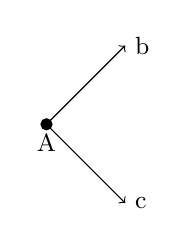
\begin{tikzpicture}
		\node[below] at (0,0) {\small$\mathrm{A}$};
		\draw[fill=black] (0,0) circle (2pt);
		\node[right] at (1,1) {\small$\mathrm{b}$};
		\draw[->] (0,0) -- (1,1);
		\node[right] at (1,-1) {\small$\mathrm{c}$};
		\draw[->] (0,0) -- (1,-1);
	\end{tikzpicture}
	\caption{Example drawing of the $\mathrm{A}\to\mathrm{b+c}$ two body decay}
	\label{fig:weaktwobody}
\end{figure}
For this decay we have
\begin{equation*}
	\sqrt{s}=M_A=\sqrt{(p^\mu p_\mu)_a+(p^\mu p_\mu)_c}
\end{equation*}
This $\sqrt{s}$ is well determined since for $\Gamma\to0$ $\abs{\varphi}^2=\delta(E-m)$.\\
We continue by writing the unstable state as a weak perturbation $\opr{\ham}_I$ on a Hamiltonian $\opr{\ham}_0$ for which the TISE holds for the unperturbed state $\ket{n}$
\begin{equation*}
	\opr{\ham}_0\ket{n}=E_n\ket{n}
\end{equation*}
We suppose that $\ket{n}$ is an orthonormal eigenvector basis for this Hamiltonian, and we begin evaluating the new perturbed state using undetermined coefficients which depend on time, after evolving the unperturbed state
\begin{equation*}
	\begin{aligned}
		\opr{\ham}\ket{\psi}&=\left( \opr{\ham}_0+\opr{\ham}_I \right)\ket{\psi}=\opr{E}\ket{\psi}\\
		\ket{\psi}&=\sum_na_n(t)\Ut\ket{n}
	\end{aligned}
\end{equation*}
We proceed by inserting the new state inside a TDSE, using $\opr{E}=i\del_t$, getting
\begin{equation*}
	\opr{E}\ket{\psi}=i\sum_n\dot{a}_n\Ut\ket{n}+\sum_na_n(t)E_n\Ut\ket{n}=\opr{\ham}\ket{\psi}
\end{equation*}
Using the first result on the unperturbed Hamiltonian and $\opr{\ham}=\opr{\ham}_0+\opr{\ham}_I$ we have immediately confronting the two results that
\begin{equation*}
	i\sum_n\dot{a}_n(t)\Ut\ket{n}=\opr{\ham}_I\ket{\psi}
\end{equation*}
Using the orthonormality of $\ket{n}$ ($\bra{k}\ket{n}=\delta_{nk}$), we have by multiplying both sides by $\bra{k}$ that
\begin{equation*}
	i\sum_n\dot{a}_n(t)\Ut\bra{k}\ket{n}=\bra{k}\opr{\ham}_I\ket{\psi}=\sum_na_n(t)\bra{k}\opr{\ham}_I\Ut\ket{n}
\end{equation*}
Rearranging things and evaluating the sums, and defining $\bra{n}\opr{\ham}_I\ket{n}=\opr{V}_{nk}$ we have
\begin{equation*}
	i\dot{a}_n(t)e^{-iE_kt}=\sum_na_n(t)\opr{V}_{nk}e^{-iE_nt}
\end{equation*}
We define for convenience $\opr{\mathcal{M}}=-i\opr{V}$, which gives us the final differential equation for the variation
\begin{equation}
	\dv{a_k}{t}=\opr{\mathcal{M}}_{kn}e^{-i(E_n-E_k)t}
	\label{eq:finalevalddeq}
\end{equation}
Where
\begin{equation}
	\opr{\mathcal{M}}_{kn}=\bra{k}\opr{\mathcal{M}}\ket{n}=-i\bra{k}\opr{V}\ket{n}=-i\bra{k}\opr{\ham}_I\ket{n}
	\label{eq:transmatrixdef}
\end{equation}
Considering that the perturbation is small we can say without problems that $a_n(0)=\delta_{mk}$ for some initial state $m$, and considering a weak time dependence, we can also say that $a_m(t)\approx1$\\
With these hypotheses $\opr{\mathcal{M}}_{mk}$ can be considered weakly dependent on time (adiabatic) and the integration will give
\begin{equation*}
	a_k(t)=\opr{\mathcal{M}}_{mk}\int_{0}^{T}e^{i(E_k-E_m)t}\dd t
\end{equation*}
Taking $k$ as our final state and $m$ our initial state the transition probability per unit time will be
\begin{equation}
	P_{i\to f}=\lim_{T\to\infty}\frac{\abs{a_f(t)}^2}{T}
	\label{eq:gammatransprobdef}
\end{equation}
Which is
\begin{equation*}
	\lim_{T\to\infty}\frac{\abs{\opr{\mathcal{M}}_{mk}}^2}{T}\int_{0}^{T}e^{i(E_f-E_i)t}\dd t\int_{0}^{T}e^{-i(E_f-E_i)\tau}\dd\tau
\end{equation*}
Executing a change of variables $T\to T-T/2$ the integrals on the right become easily identifiable as the Fourier transforms of a complex exponential, which gives $\hat{f}(x)=2\pi\delta(x)$, and therefore
\begin{equation*}
	P_{i\to f}=\lim_{T\to\infty}\frac{\abs{\opr{\mathcal{M}}_{mk}}^2}{T}2\pi T\delta(E_f-E_i)
\end{equation*}
Which finally gives \emph{Fermi's golden rule} for time dependent perturbations
\begin{equation}
	P_{i\to f}=2\pi\abs{\opr{\mathcal{M}}_{mk}}^2\delta(E_f-E_i)
	\label{eq:fermigoldenruledecay}
\end{equation}
Since there are various possibilities for this two body decay, it's necessary to then consider a statistical approach for the energies, and we need to evaluate the density of states in the phase space, for the volume $E_f-E_i$. In this case, considering then all possible decays, we have finally the transition rate between the initial and the final state
\begin{equation*}
	\Gamma_{fi}=\int_{}^{}P_{i\to f}\dd n=\int_{}^{}P_{i\to f}\dv{n}{E_f}\dd E_f=2\pi\abs{\opr{\mathcal{M}}_{fi}}^2\int_{}^{}\delta(E_f-E_i)\dv{n}{E_f}\dd E_f
\end{equation*}
Integrating the delta on the right we have finally
\begin{equation}
	\Gamma=2\pi\abs{\opr{\mathcal{M}}_{fi}}^2\rho(E_i)
	\label{eq:decayratefinal}
\end{equation}
Where $\opr{\mathcal{M}}_{fi}$ depends on the interaction Hamiltonian, whereas $\rho(E_i)$ is the density of states in the phase space for the two body decay.
\subsection{Beta Decay Rate}
Using what we found before for unstable states we can immediately imagine to apply it to Fermi's theory of $\beta$ decay. In this case we have a reaction of the type
\begin{equation*}
	n\to p+e^-+\cc{\nu}
\end{equation*}
Here, we have $\ket{i}=\ket{n}$ and $\ket{f}=\ket{pe^-\cc{\nu}}$. The decay rate as for Fermi's golden rule is
\begin{equation*}
	\Gamma=2\pi\abs{\opr{\mathcal{M}}_{fi}}^2\rho(E)
\end{equation*}
Where, in this case
\begin{equation}
	\opr{\mathcal{M}}_{fi}=-i\int_{}^{}\cc{\psi}_p\cc{\psi}_e\cc{\psi}_\nu G_F\psi_n\dd^3r
	\label{eq:fermidecay}
\end{equation}
Where $G_F$ is our interaction parameter.\\
Suppose to normalize the wavefunctions on a nuclear volume $V$, $\psi\propto V^{-1/2}$. With this normalization we also have that $[G_F]=E^{-2}$.\\
Considering the total decay the wavefunctions for $e^-,\cc{\nu}$ can be considered without loss of generality as plane waves due to their non-interacting nature after the decay, therefore
\begin{equation}
	\begin{aligned}
		\psi_e&=\frac{1}{\sqrt{V}}e^{-i\vec{p}\vec{r}}\\
		\psi_\nu&=\frac{1}{\sqrt{V}}e^{-i\vec{q}\vec{r}}
	\end{aligned}
	\label{eq:electronneutrinowf}
\end{equation}
Where we chose $\vec{p}_e=\vec{p}$ and $\vec{p}_\nu=\vec{q}$.\\
Approximating the interaction factor $G_F$ as a constant as for Fermi's theory we have finally
\begin{equation*}
	\opr{\mathcal{M}}_{fi}=-i\frac{G_F}{V}\int_{}^{}\cc{\psi}_p\psi_ne^{i(\vec{p}+\vec{q})\vec{r}}\dd^3r
\end{equation*}
Another approximation can be made by checking that $Q=m_n-m_p-m_e-m_\nu\le1$ and therefore $p\simeq q\le1\unit{MeV}$, and $r\approx1\unit{fm}$, which gives $(p+q)r\approx5/1000$.\\
Considering this the exponential in this integral can be expanded with a power series and approximated to the first order, giving
\begin{equation}
	\opr{\mathcal{M}}_{fi}=-i\frac{G_F}{V}\int_{}^{}\cc{\psi}_p\psi_n\dd^3r=-\frac{iG_FN}{V}
	\label{eq:transmatrixfermidec}
\end{equation}
Where $N$ is the so called \emph{nuclear term} $N=\bra{p}\ket{n}$.\\
Reinserting it into the decay rate equation we have
\begin{equation*}
	\Gamma=\frac{2\pi G_F^2\abs{N}^2}{V^2}\rho(E)
\end{equation*}
We only need to find $\rho(E)$ in order to complete the calculations. Considering that for the conservation of 3-momentum $\vec{p}_e+\vec{p}_\nu+\vec{p}_X=0$, and for the conservation of energy
\begin{equation}
	\begin{aligned}
		\rho(E)&=\left(\dv{n}{E_f}\right)_{E_i}=\int_{}^{}\delta(E_f-E_i)\dd n\\
		\dd n&=\frac{V^2}{(2\pi)^6}\dd^3p\dd^3q
	\end{aligned}
	\label{eq:densitycalc}
\end{equation}
In the center of mass of X we have then
\begin{equation*}
	E_i=\sqrt{s}=M_X,\quad E_f=E_Y+E_e+E_\nu=M_Y+K_Y+E_e+E_\nu
\end{equation*}
Considering that the masses of X and Y are much greater than the mass of the electron and neutrino we have that $K_Y\approx0$ and we have $M_X\approx M_Y+E_e+E_\nu$. The total available energy for the reaction will then be
\begin{equation*}
	E_T=M_X-M_Y=E_e+E_\nu
\end{equation*}
And, therefore
\begin{equation*}
	Q=M_X-M_Y-m_e-m_\nu\approx E_T
\end{equation*}
In the limit case where $\mathrm{X}=p$ and $\mathrm{Y}=n$ we have $E_T\approx1\unit{MeV}$, and
\begin{equation*}
	\delta(E_f-E_i)=\delta(E_T-E_e-E_\nu)
\end{equation*}
Approximating $m_\nu=0$ we have $E_\nu=q$ and therefore $q^2\dd q=E_\nu^2\dd E_\nu$. For the electron we have instead
\begin{equation*}
	p=\sqrt{E_e^2-m_e^2}\qquad p^2\dd p=pE_e\dd E_e
\end{equation*}
Substituting in the delta integral we have
\begin{equation*}
	(4\pi)^2\iint\delta(E_f-E_i)p^2q^2\dd p\dd q=(4\pi)^2\iint\delta(E_T-E_e-E_\nu)E_\nu^2E_ep\dd E_\nu\dd E_e=(4\pi)^2\int_{0}^{E_T}pE_e(E_T-E_e)^2\dd E_e
\end{equation*}
Substituting $p$ we get finally for the decay rate
\begin{equation*}
	\Gamma_\beta=\frac{G_F^2\abs{N}^2}{2\pi^3}\int_{0}^{E_T}E_e\sqrt{E_e^2-m_e^2}(E_T-E_e)^2\dd E_e
\end{equation*}
For the limit case of a hyperrelativistic electron we can say with ease that $m_e<<E_e$ and therefroe we can approximate the integral as follows
\begin{equation*}
	\int_{0}^{E_T}E_e^2(E_T-E_e)^2\dd E_e=\frac{E_T^5}{3}+\frac{E_T^5}{5}-\frac{E_T^5}{2}
\end{equation*}
Summing up and inserting into the decay rate we get \emph{Sargent's rule} for beta decay with highly energetic electrons
\begin{equation}
	\Gamma=\frac{G_F^2\abs{N}^2}{60\pi}E^5_T
	\label{eq:sargentrule}
\end{equation}
Since here $E_T\approx M_X-M_Y$ we have that the phase space must grow with $M_X-M_Y$
\subsection{Experimental Estimate of $m_\nu$}
So far the hypotheses we managed to stack up from beta decay are
\begin{enumerate}
\item $m_\nu\ne0$
\item $\Gamma\propto pE_e(E_T-E_e)^2$, $E_T=M_X-M_Y-m_\nu-m_e=E_e+E_\nu$
\end{enumerate}
It's clear that reducing $E_T$ we have the maximum possible $E_e$. We define here the Kurie function $K(E)$ as
\begin{equation*}
	K(E)=\sqrt{\frac{1}{pE_e}\dv{\Gamma}{E}}\propto(E_T-E_e)^2
\end{equation*}
Evaluating this function for a minimal $E_T$ it's possible to resolve $E_T-m_\nu$ and evaluate the neutrino mass.\\
Note that $K(E)\propto(E_T-E_e)$ and therefore we expect a linear decay of this function up until $E_e^{max}$. Experimentally it has been observed that at $\min(E_T)$ instead the function evaluates to $E_T-m_\nu$ effectively giving an estimate for the mass of the neutrino
\subsection{Cross Section for Beta Decays}
The reaction considered up until now
\begin{equation*}
	n\to p+e^-+\cc{\nu}
\end{equation*}
Can also be reversed, indicating that another weak reaction is possible
\begin{equation}
	\cc{\nu}+p\to n+e^+
	\label{eq:neutrinoprotonscattering}
\end{equation}
This scattering reaction is experimentally observed, but we must
\begin{itemize}
\item generate neutrinos
\item choose a $p$-rich target
\item observe $n,e^+$ and count the number of events
\item measure the scattering cross section $\sigma$
\end{itemize}
The first question we get is: Can Fermi's 4-fermion theory evaluate theoretically $\sigma$?\\
Starting again from cross sections we have, by definition that the number of observed reactions per unit time is
\begin{equation*}
	\dv{N_R}{t}=\sigma n_T\dv{N_p}{t}\dd x
\end{equation*}
Where $N_p$ is the number of incoming projectiles, and $n_T$ is the particle density of the target.\\
Evaluating everything we have
\begin{equation*}
	\dv{N_R}{t}=\frac{\sigma}{S}\underbrace{n_TS\dd x}_{N_T}
\end{equation*}
Also using $S^{-1}\dd N_p/\dd t=\phi_p$, i.e. the flux of incoming projectiles, we have
\begin{equation*}
	\frac{1}{N_T}\dv{N_R}{t}=\sigma\phi_p=\sigma v_pn_p=\sigma\frac{N_p}{V}
\end{equation*}
Where $n_p,N_p$ are respectively the number density and total number of particles of the projectile beam, and $v_p$ is the relative velocity of the projectiles with respect to the target.\\
Fixing the previous equation we have
\begin{equation*}
	\frac{1}{N_TN_p}\dv{N_R}{t}=\sigma\frac{v_p}{V}
\end{equation*}
Using $v_p=p_p/E_p$ and noting that on the left we have the number of reaction per unit time per single projectile on a single target, we have
\begin{equation*}
	\frac{1}{N_TN_p}\dv{N_R}{t}=\sigma\frac{p_p}{VE_p}=\Gamma(a+b\to c+d)=2\pi\abs{\opr{\mathcal{M}}_{fi}}^2\rho(E)
\end{equation*}
Therefore we have
\begin{equation}
	\sigma(a+b\to c+d)=2\pi\abs{\opr{\mathcal{M}}_{fi}}^2\frac{V}{v_p}\rho(E)
	\label{eq:sigmafermirule}
\end{equation}
For our reaction we have the following scattering reaction
\begin{figure}[H]
	\centering
	\begin{tikzpicture}
		\node[left] at (-2,0) {$\cc{\nu}$};
		\draw[fill=black] (0,0) circle (1pt);
		\node[below] (0,0) {$p$};
		\draw[->] (-2,0) -- (-0.2,0);
		\draw[->] (0.2,0.2) -- (1,1) node[right] {$e^+$};
		\draw[->] (0.2,-0.2) -- (1,-1) node[right] {$n$};
	\end{tikzpicture}
	\caption{Scattering process in study}
	\label{fig:protonneutrinoscatter}
\end{figure}
Moving to the center of mass of the initial $\cc{\nu}+p$ state we have
\begin{equation*}
	\beta\gamma=\frac{p}{\sqrt{s}}=\frac{E_\nu}{\sqrt{m_p^2+2E_pm_\nu}}
\end{equation*}
Where we approximated $m_\nu=0$ therefore $p_\nu=E_\nu$.\\
The velocity of the $\nu$ with respect to the $p$ targets is therefore
\begin{equation*}
	v_i=\frac{p_\nu^\star}{E_\nu^\star}+\frac{p_p^\star}{E_p^\star}
\end{equation*}
Inserting it all into the cross-section equation we get
\begin{equation*}
	\sigma=\frac{2\pi G_F^2\abs{N}^2}{V}\frac{E_\nu^\star E_p^\star}{p_\nu^\star E_p^\star+p_p^\star E_\nu^\star}\rho(E_f)
\end{equation*}
In order to calculate the density of states in the final decayed state we need to consider the conservation of 3-momentum, which implies $p^\star_n=p^\star_e=p^\star$, and accounting that
\begin{equation*}
	\rho(E_f)=\dv{n}{E_f}=\frac{V}{2\pi^2}p^2\dv{p}{E_f}
\end{equation*}
Using $E_f=\sqrt{p^2+m_e^2}+\sqrt{p^2+m_n^2}$ gives
\begin{equation*}
	\dv{E_f}{p^\star}=\frac{p(E_n^\star+E_e^\star)}{E_n^\star E_e^\star}=v_f
\end{equation*}
Where $v_f$ is the velocity of the positrons with respect to the neutrons. Inverting and inserting it into the cross-section equation, using $E_f=E_n^\star+E_e^\star$ we have
\begin{equation}
	\sigma=\frac{G_F^2\abs{N}^2(p^\star)^2}{\pi v_i v_f}=\frac{G_F^2\abs{N}^2}{\pi}\frac{E_p^\star E_\nu^\star E_p^\star E_e^\star}{E_f\left(p_\nu^\star E_p^\star+p_p^\star E_p^\star\right)}p^\star
	\label{eq:crossecbeta}
\end{equation}
Where $p^\star=p^\star_e=p^\star_\nu$ is the momentum of the final two decay products, the positron and the neutron.\\
Inserting the experimental values of $G_F=1.17\cdot10^{-5}\unit{GeV^{-2}}$, $v_i\approx v_f\approx1$, we get
\begin{equation*}
	\sigma (p^\star)^2\approx10^{-37}\unit{cm^2/GeV^2}
\end{equation*}
Considering that the $Q-$value for this reaction is $Q\approx1.8\unit{MeV}$ we have that this process is possible only if $E_\nu>1.8\unit{MeV}$ which gives, for the cross-section at threshold level
\begin{equation*}
	\sigma (p^\star)^2\approx10^{-43}\unit{cm^2/GeV^2}
\end{equation*}
In order to evaluate what it means for experimental tests of this decay we need to account for the mean free path of the reaction. Supposing a light water target, for which $A_{\mathrm{H_2O}}=18\unit{g/mol}$ we have $n_T=A^{-1}N_A$, for which we get
\begin{equation*}
	\frac{1}{\lambda}=\sigma n_T=E\cdot10^{-43}\cdot 3\cdot10^{22}\unit{MeV^{-1}cm^{-1}}
\end{equation*}
Using $E\approx1\unit{MeV}$ we get an estimate of $\lambda\approx10^{19}m$ which is an absurdly large mean free path for such reaction.\\
What is needed therefore for building experiments on this reaction is to note that accelerated neutrinos will have a higher $E_\nu$, and therefore will contribute to lower this. A second fix is the usage of high density targets together with heavy neutrinos emitters.\\
One way of accomplish this is considering Uranium fission. In 1956 Reines, Cowen et al. were the first to build a nuclear reactor for the production of energy, with a thermal power output of $1000\unit{MW}=10^9\unit{J/s}=6\cdot10^{27}\unit{eV/s}$.\\
Considering $Q_{fis}=200\unit{MeV}$ and a production of around $N_\nu=6$ neutrinos per reaction we have
\begin{equation*}
	N_R=\frac{P_{reactor}}{Q}=3\cdot10^{19}\unit{Hz}
\end{equation*}
Which implies an average production of $10^{20}\unit{Hz}$ neutrinos, with $E_\nu\approx3\unit{MeV}$.\\
Not too far from the reactor core we have that the flux of neutrinos per solid angle of detector is
\begin{equation*}
	\phi_\nu=\frac{\dd N_\nu}{\dd t\dd S}=10^{13}\unit{cm^{-2}s^{-1}}
\end{equation*}
Using a $\mathrm{CaCl_2+H_2O}$ target the reaction we expect to observe is an extra production of $\gamma+\gamma$ corresponding to the following reaction between the decay products and the electrons of the target
\begin{equation*}
	\begin{aligned}
		\cc{\nu}+p&\to n+e^+\\
		e^++e^-&\to\gamma+\gamma
	\end{aligned}
\end{equation*}
There is a second $\gamma+\gamma$ peak that needs to be accounted, since neutrons thermalize in the collisions with the fluid, it's possible to also have a neutron capture reaction inside the target, as follows
\begin{equation*}
	n+\nuc{X}{A}{Z}\to\nuc{Y^\star}{A+1}{Z}\to\nuc{Y}{A+1}{Z}+\gamma+\gamma
\end{equation*}
Where $E_\gamma\approx6\unit{MeV}$. Turning on the reactor it's possible to see a sharp increase of $\gamma+\gamma$ reactions, corresponding to the neutrino scattering, confirming the existence of the neutrino.
\end{document}
